\documentclass[12pt]{article}
\usepackage[utf8]{inputenc}
\usepackage{amsmath}
\usepackage{graphicx}
\graphicspath{ {./} }
\setlength{\parskip}{1em}

\title{Week 4 Questions}
\author{tprasad@tcd.ie 16326505}
\pagenumbering{gobble}
\begin{document}
\maketitle
\begin{flushleft}
Question 1

	(a) \{(1,1)\}
	
	(b)	\{(1,1),(2,1),(1,2)\}
	
	(c)	\{(1,3),(3,1),(2,2)\}
	
	(d) \[ \frac{3}{6^2} = 0.08333 \]
	
Question 2

	(a)	-3,-1,1,3
	
	(b) \[ \{(T,T,T)\} = \frac{1}{2^3} = 0.125 \]
	
	(c) \[\{(H,T,T),(T,H,T),(T,T,H)\} = 0.375\]
	
	(d)	Probability of P(X=1) = P(X=-1) and same for P(X=3) and 	P(X=-3)
	
	PMF = plotting out these values =
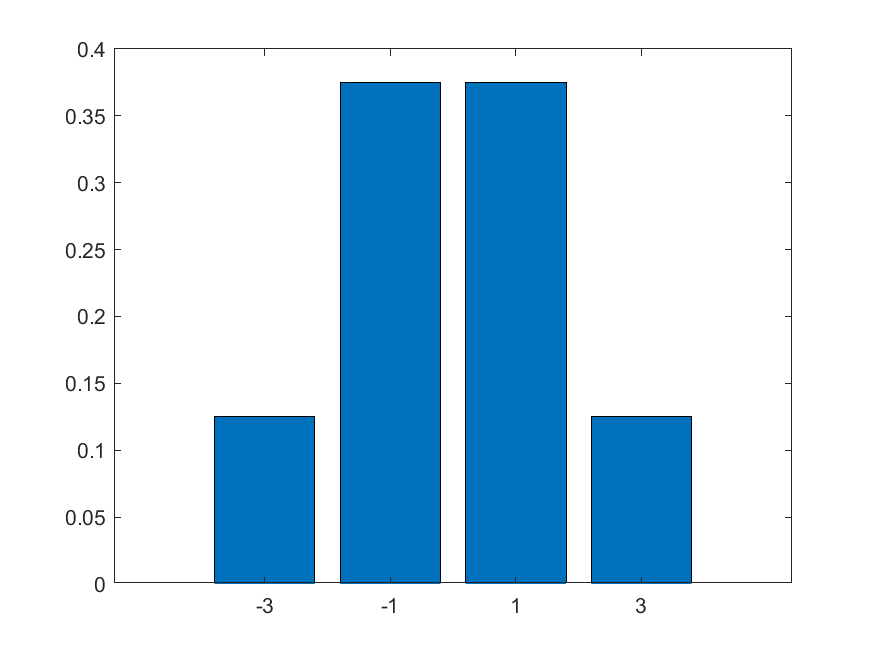
\includegraphics[scale=1]{PMF}

	CDF =
		\[ -3 = .125 \]
		\[ -1 = .375 + .125 = .5\]
		\[ 1 = .875 \]
		\[ 3 = 1 \]
		
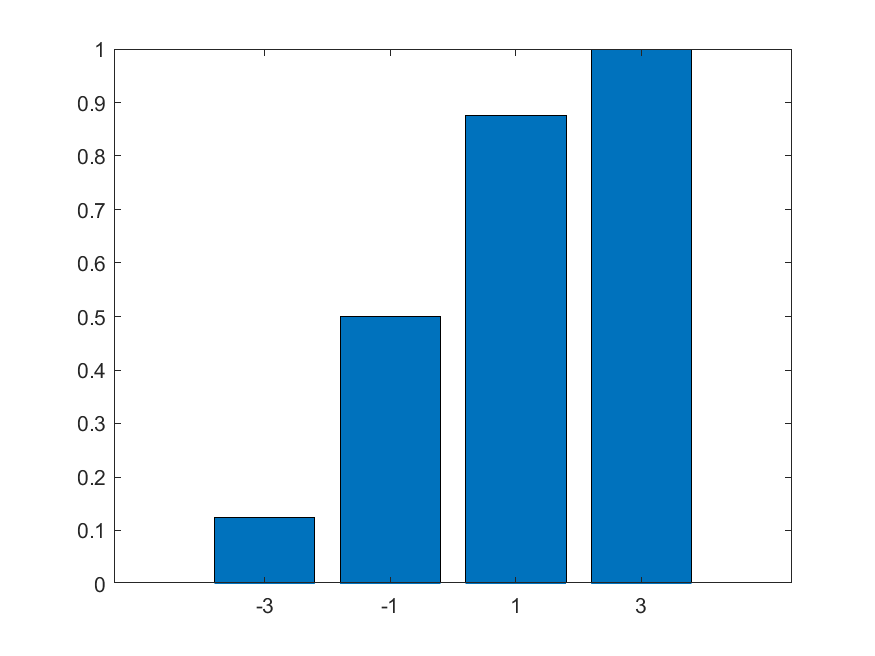
\includegraphics[scale=1]{Barchart}
		
	
		
Question 3

	(a) 1 since all numbers on the dice are $>= 1$
	
	(b) $ \left(\frac{5}{6}\right)^4 = 0.4823$ since exactly 1 possibility in 6 can't be landed on all 4 times
	
	(c)	1 for all 

	
\end{flushleft}
\end{document}